\chapter{SCATTERING THEORY}
\section{The Scattering Cross Section}
A parallel beam of particle of given momentum is directed towards a target which deflects or scatters the particle in various directions.The scattered particles diverge. Eventually at large distance from the target, their motion is directed radially outwards.It is convenient to choose a system with the origin at the position of the target or scattering center. and with Z-axis in the direction of the incident beam .The direction of any scattered particle is indicated by polar angles ($\theta, \phi$) with the z-axis taken as the polar axis.Then $\theta$ is the angle of scattering ie the angle between the scattered and the incident direction .These two directions together define the plane of scattering .The azimuthal angle $\phi$ specifies the orientation of the this plane with respect to some reference plane containing z-axis.\\
\begin{figure}[H]
	\centering
	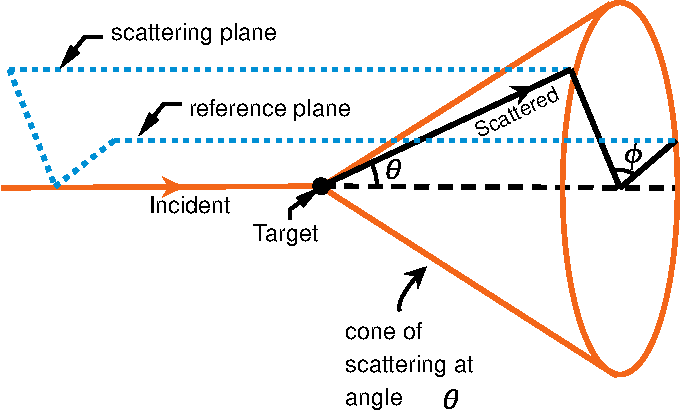
\includegraphics[height=4.8cm,width=8cm]{diagram-20220131-crop}
	\caption{}
	\label{}
\end{figure}
\par Let the incident flux F is independent of time.There will then be steady stream of particles too.Let $\Delta N$ be the number of particles scattered in to a small solid angle $\Delta \Omega$ about the direction $(\theta \phi)$ in time $\Delta t$.Evidently 
$\Delta N$ must be proportional to $\Delta \Omega \Delta t$ and to the incident flux F.The proportionality factor which depends in general on $\theta$ and $\phi$ is called the differential scattering cross section, and is denoted by ($\frac{d\sigma}{d\Omega}$)\\
$$ \Delta N=\frac{d\sigma(\theta,\phi)}{d\Omega}\Delta t \Delta \Omega F$$
$\frac{d\sigma}{d\Omega}$ has a dimension of area,it depends only on the parameters of the incident particle and nature of the target.\\
The total scattering crosssection $\sigma$ may be obtained from it by integration over all directions:\\
$$\sigma=\int (\frac{d\sigma}{d\Omega})d\Omega=\int_{0}^{2\pi}\int_{0}^{\pi}(\frac{d\sigma}{d\Omega})\sin \theta d\theta d\phi$$
In most cases we consider ($\frac{d\sigma}{d\Omega}$) is independent of $\phi$\\
Then $$\sigma=\int (\frac{d\sigma}{d\Omega}) 2\pi \sin \theta d \theta$$
\subsection{The Scattering Amplitude}
When the particle involved in the scattering process are quantum mechanical objects ,we must describe them by a wave function.At large distance from the scattering centre ($r\rightarrow \infty$) the form of the wavefunction must consist of a part $u_{inc}$ corresponding to the parallel beam of incident particles and the other part $u_{sc}$ representing the scattered particle moving radially outwards from the center.\\
$$u(\mathbf{x}) \underset{r \rightarrow \infty}{\longrightarrow} u_{i n c}+u_{s c}$$
The beam of incident particles with momentum $p=\hbar k$ along the $z$-axis must evidently be described by the plane wave (momentum eigenfunction) $u_{i n c}=e^{i k z}$.\\
 $\left\lfloor\left. u_{\text {inc }}\right|^{2}\right.$ is to be understood as the number of incident particles per unit volume. The incident flux is obtained by multiplying this quantity by the particle velocity $v$.
$$
F=\left|u_{\text {inc }}\right|^{2} v=\hbar k / m
$$ 
Suppose that the scattering is elastic. Then the wave $u_{s c}$ representing them must have the same propagation constant $k_{i}$ but it must be a spherical wave since these particles move radially. The only such waves are $e^{i k r}$ and $e^{-i k r}$; the latter is an incoming wave (contracting towards the origin). Since the scattercd particles move outwards, we must choose the outgoing wave $_{2} u_{s c} \propto e^{i k r}$. Further, the flux of scattered particles, $\left|u_{s c}\right|^{2}(\hbar k / m)$ must evidently decrease as $\left(1 / r^{2}\right)$ as $r$ increases. Hence $u_{s c} \propto(1 / r)$ also, and we writê
$$
u_{s c}=f(\theta, \varphi) \frac{e^{i k r}}{r}
$$
The dependence of the proportionality factor $f$ on $\theta, \varphi$ allows for the fact that the scattered flux is, in gencral, direction-dependent. We observe now that $\triangle \mathcal{N}$ is nothing but the radial flux times $\triangle S \Delta t$, where $\Delta S \equiv r^{2} d \Omega$ is the element of area (normal to the radial direction) covered by the solid angle $\Delta \Omega$. Thus
$$
\begin{aligned}
\Delta \mathcal{N} &=\left|u_{s c}\right|^{2}(\hbar k / m) \cdot r^{2} \Delta \Omega \Delta t \\
&=|f(\theta, \varphi)|_{0}^{2}(\hbar k / m) \Delta \Omega \Delta t
\end{aligned}
$$
On substituting this together with $F=\frac{\hbar k}{m}$ in $ \Delta N=\frac{d\sigma(\theta,\phi)}{d\Omega}\Delta t \Delta \Omega F$, we obtain\\
$$\frac{d \sigma(\theta, \varphi)}{d \Omega}=|f(\theta, \varphi)|^{2}$$\\
\textbf{$f(\theta, \varphi) \text { is called the scattering amplitude. }$}\\
The particular stationary  wavefunction can be written as \\
$$u(\mathbf{x}) \underset{r \rightarrow \infty}{\longrightarrow} e^{i k z}+f(\theta, \varphi) \frac{e^{i k r}}{r}$$
Since any stationary wave function must satisfy the time independent Schrcdinger equation, we must have
$$
-\frac{\hbar^{2}}{2 m} \nabla^{2} u(\mathbf{x})+V(\mathbf{x}) u(\mathbf{x})=E u(\mathbf{x}), \quad E=\frac{\hbar^{2} k^{2}}{2 m}
$$
Here $V(\mathbf{x})$ is the potential energy function for the projectile particle in the force field of the scattering centre. \\\\
\textbf{Formal Expression for Scattering Amplitude}
$$\begin{aligned}
	f(\theta, \varphi) &=-\frac{1}{4 \pi} \int e^{-i \mathbf{k} \cdot \mathbf{x}} U(\mathbf{x}) u(\mathbf{x}) d \tau, \\
	&=-\frac{m}{2 \pi \hbar^{2}} \int e^{-i \mathbf{k} \cdot \mathbf{x}} V(\mathbf{x}) u(\mathbf{x}) d \tau
\end{aligned}$$
\subsection{First Born Approximation}
$$f(\theta, \varphi)=-\frac{1}{4 \pi} \int e^{-i \mathbf{k} \cdot \mathbf{x}} U(\mathbf{x}) u(\mathbf{x}) d \tau$$
Suppose that $\left|u(\mathbf{x})-e^{i k z}\right|<\left|e^{i k z}\right|=1$\\
Then we can replace the unknown $u(\mathbf{x})$ in $f(\theta, \varphi)$ to a good approximation, by $e^{i k z} \equiv e^{t \mathbf{k}_{0} \cdot \mathbf{x}}$ where $k_{0}$ is the vector of magnitude $k$ in the incident direction. The resulting expression is called the \textbf{first Born approximation} to $f(\theta, \varphi)$ and is given by
$$
f_{\mathrm{H}}(\theta, \varphi)=-(4 \pi)^{-1} \int e^{-i \mathbf{K} \cdot \mathbf{x}} U(\mathbf{x}) d \tau \text {. }
$$
The scattering. cross-scction in this approximation is
$$
\left(\frac{d \sigma}{d \Omega}\right)_{\mathrm{B}}=(4 \pi)^{-2}\left|\int e^{-i} \mathbf{K} \cdot \mathbf{x} U(\mathbf{x}) d \tau\right|^{2} .
$$
In equation $f_{\mathrm{H}}(\theta, \varphi)$  $\mathbf{K}=\mathbf{k}- \mathbf{k}_{0}$. It may be noted that $\hbar \mathbf{K}$ is the momentum transferred to the particle in its encounter with the potential. Since $\left|k_{0}\right|=|\mathbf{k}|$ $=k$, it follows (from the figure )that
$$K \equiv|\mathbf{K}|=2 k \sin \frac{1}{2} \theta$$
\begin{figure}[H]
	\centering
	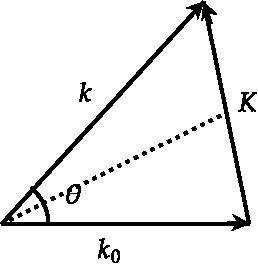
\includegraphics[height=2.7cm,width=3.5cm]{nimi1-crop}
	\caption{}
	\label{}
\end{figure}
The scattcring amplitude in the Born approximation, considered as ifunction of $\mathrm{K}$ : is the Fourier transform of the potcntial (apart from constant facturs;)\\
In the most important special case when V is sphcrically symmetric, $V(\mathbf{x})$ - V $(r)$, we can reduce $
f_{\mathrm{H}}(\theta, \varphi)$ to an integral over $r$ alone, by going over to spherical polar coordinates $(r, \alpha, \beta)$ with the direction of $\mathbf{K}$ chosen as the polar axis. Then $\mathbf{K} . \mathbf{x}=K_{r} \cos \alpha$ and on carrying out the angular integrations one $\operatorname{gcts}$
$$
f_{B}(\theta)=-K^{-1} \int_{0}^{\infty} r \sin K r U(r) d r
$$
\subsection{Partial Wave Analysis}
While the Born approximation is basically a truncation of a perturbation expansion of $u(x)$, the method of partial waves is based upon an expansion of $u(\mathbf{x})$ in terms of angular momentum eigenfunctions. It is applicable if the potential is spherically symmetric. one gets a fornial expression for the scattering amplitude as an infinite scries; cach term of the series is the contribution to $f(\theta, \varphi)$ from a partial wave characterized by a particular angular momentum. We shall see that the first few terms in the series approximate $f(\theta, \varphi)$ if the incident particle is of low energy. Thus the partial wave method leads to a low energy approximation which complements the Born approximation (good at high energies).
\subsubsection{Partial Waves}
If the potential has sphencal symmetry we can separate the Schrödinger equation into radial and angular parts, and obtain solutions in the form $R_{l}(r) Y_{l m}{(\theta, \varphi)}$, where the radial wave functions $R_{l}(r)$ satisfy the equation
$$
1/r^2 \frac{d}{dr}\left(r^{2} \frac{d R_l}{d r}\right)+\frac{2 \mu}{\hbar^{2}}\left[E-V-\frac{l(l+1) \hbar^{2}}{2 \mu r^{2}}\right] R_l=0
$$
The general solution of the Schrödinger equation can be written as a linear combination of such solutions. In the scattering problem which we are considering, only the function $R_{l}(r) \bar{\gamma}_{l o}(\theta, \varphi) \propto R_{l}(r) P_{l}(\cos \theta)$ appears in the linear combination. This is because we have assumed the particle to be travelling in the $z$-direction initially, so that the $z$-component of its angular momentum is zero; it continues to be zero because a spherically symmetric potential does not disturb the angular momentum. Thus we can write
$$
u(\mathbf{x})=\sum_{l=0}^{\infty} R_{l}(r) P_{l}(\cos \theta)
$$
The term corresponding to a particular $l$ in this series is called the lth partial wave.\\\\
\textbf{Asymptotic Form of Radial Function}\\
 We must now require that $u(\mathbf{x})$ should have the asymptotic form of$u(\mathbf{x}) \underset{r \rightarrow \infty}{\longrightarrow} e^{i k z}+f(\theta, \varphi) \frac{e^{i k r}}{r}$ \\
  This condition places constraints on the radial wave functions $R l(r)$. To see what they are, we need to have the asymptotic $(r \rightarrow \infty)$ form of $R_{l}(r)$. We can infer it from the radial wave equation  which we rewrite as
$$
\left.\begin{array}{l}
\frac{d^{2} \chi_{l}}{d r^{2}}+\left[k^{2}-U(r)-\frac{l(l+1)}{r^{2}}\right] \chi_{l}=0, \\
\chi_{l}=r R_{l}(r), k^{2}=\left(2 m E / \hbar^{2}\right), U(r)=2 m V / \hbar^{2}
\end{array}\right\}
$$
In the asymptotic region, both $U(r)$ and the centrifugal potential $\left(\propto 1 / r^{2}\right)$ are very small. On neglecting these, in comparison with $k^{2}$, we obtain the approximate asymptotic solution $\chi_{l}(r) \propto e^{\pm i k r}$. To improve this approximation, let us suppose that
$$\chi_{l}(r)=v_{l}(r) e^{\pm i k r}$$
where $v_{l}(r)$ is expected to be very slowly varying in the asymptotic region. On introducing this into Eq in to new radial equation we get
$$
d^{2} v_{l} / d r^{2} \pm 2 i k d v_{l} / d r-\left[U+l(l+1) / r^{2}\right] v_{l}=0
$$
on solving this we will get\\
$$\ln v_{l} \approx \mp \frac{i}{2 k} \int^{r}\left[U+\frac{l(l+1)}{r^{2}}\right] d r$$
\textcolor{red}{some text missing} if $1/r$ is large enough the value of the integral is effectively independent of $r$ and hence $v_{l}(r)$ is a constant in the asymptotic region. In the following, we will confine our attention to such potentials, leaving the Coulomb case to be dealt with later. Then the asymptotic form of $\chi_{l}(r)$ is, in general, some linear combination of the two solutions with $v_{l}$ constant, i.e. of $e^{i k r}$ and $e^{-ikr}$. Without loss of generality, we can write any such combination in the form\\
$${\chi}_{l} \rightarrow C_{l} \sin \left(k r+\Delta_{l}\right)$$
$\text { where } C_{l}, \Delta_{l} \text { are constants. }$\\\\
\textbf{Phase Shift}\\
 Let us compare the above asymptotic behaviour with that of the partial waves for a free particle $\left(V^{\prime}(r)=0\right)$. We have already seen  that in any range of $r$ over which $V(r)$ is constant, the solutions of the radial wave equation are the spherical Bessel functions $j_{l}$ or $n_{l}$. In particular, if $V=0$ everywhere, the only admissible solution is $j_{l}(k r) ; n_{l}$ is ruled out because it becomes infinite at $r=0$. Thus $R_{l}(r)=$ const. $j_{l}(k r)$ in the free-particle case. Since the asymptotic forms of the spherical Bessel functions are known to be given by
 $$\begin{aligned}
 	&j_{l}(k r) \rightarrow(k r)^{-1} \sin \left(k r-\frac{1}{2} l \pi\right) \\
 	&n_{l}(k r) \rightarrow-(k r)^{-1} \cos \left(k r-\frac{1}{2} l \pi\right)
 \end{aligned}$$
 (as $r \rightarrow \infty$ ), it follows tha $\chi_{l}(r)=r R_{l}(r) \rightarrow$ const. $\sin \left(k r-\frac{1}{2} l \pi\right)$. Hence $\chi_{l}$ in this case has the asymptotic form ${\chi}_{l} \rightarrow C_{l} \sin \left(k r+\Delta_{l}\right)$ with the particular value $-\frac{1}{2} l \pi$ for $\Delta_{l}$.\\
 The effect of the potential on the partial waves in the asymptotic region is, therefore, simply to change the phase from - $\frac{1}{2} \pi l$ to some other value $\triangle_{l}$. This change,
 $$
 \delta_{l}=\Delta_{l}+\frac{1}{2} l \pi
 $$
 is called the phase shift in the lth partial wave.
 \newpage
 \begin{abox}
 	Practice set 1
 	\end{abox}
 \begin{enumerate}
 	\begin{minipage}{\textwidth}
 	\item A free particle described by a plane wave and moving in the positive $z$-direction undergoes scattering by a potential
 	$$
 	V(r)= \begin{cases}V_{0}, & \text { if } r \leq R \\ 0, & \text { if } r>R\end{cases}
 	$$
 	If $V_{0}$ is changed to $2 V_{0}$, keeping $R$ fixed, then the differential scattering cross-section, in the Born approximation.
 	\exyear{NET JUNE 2012}
 \end{minipage}
 \begin{tasks}(1)
 	\task[\textbf{A.}]Increases to four times the original value
 	\task[\textbf{B.}]Increases to twice the original value
 	\task[\textbf{C.}]Decreases to half the original value
 	\task[\textbf{D.}]Decreases to one fourth the original value
 \end{tasks}
\begin{minipage}{\textwidth}
	\item The differential cross-section for scattering by a target is given by
	$$
	\frac{d \sigma}{d \Omega}(\theta, \phi)=a^{2}+b^{2} \cos ^{2} \theta
	$$
	If $N$ is the flux of the incoming particles, the number of particles scattered per unit time is
	\exyear{NET JUNE 2015}
\end{minipage}
\begin{tasks}(2)
	\task[\textbf{A.}] $\frac{4 \pi}{3} N\left(a^{2}+b^{2}\right)$
	\task[\textbf{B.}]$4 \pi N\left(a^{2}+\frac{1}{6} b^{2}\right)$
	\task[\textbf{C.}]$4 \pi N\left(\frac{1}{2} a^{2}+\frac{1}{3} b^{2}\right)$
	\task[\textbf{D.}]$4 \pi N\left(a^{2}+\frac{1}{3} b^{2}\right)$
\end{tasks}
\begin{minipage}{\textwidth}
	\item A particle of energy $E$ scatters off a repulsive spherical potential
	$$
	V(r)=\left\{\begin{array}{ccc}
	V_{0} & \text { for } & r<a \\
	0 & \text { for } & r \leq a
	\end{array}\right.
	$$
	where $V_{0}$ and $a$ are positive constants. In the low energy limit, the total scattering crosssection is $\sigma=4 \pi a^{2}\left(\frac{1}{k a} \tanh k a-1\right)^{2}$, where $k^{2}=\frac{2 m}{h^{2}}\left(V_{0}-E\right)>0$. In the limit $V_{0} \rightarrow \infty$ the ratio of $\sigma$ to the classical scattering cross-section off a sphere of radius $a$ is
	\exyear{NET JUNE 2015}
\end{minipage}
\begin{tasks}(4)
	\task[\textbf{A.}] 4
	\task[\textbf{B.}]3
	\task[\textbf{C.}]1
	\task[\textbf{D.}]$\frac{1}{2}$
\end{tasks}
\begin{minipage}{\textwidth}
	\item A particle is scattered by a central potential $V(r)=V_{0} r e^{-\mu r}$, where $V_{0}$ and $\mu$ are positive constants. If the momentum transfer $\vec{q}$ is such that $q=|\vec{q}| \gg \mu$, the scattering crosssection in the Born approximation, as $q \rightarrow \infty$, depends on $q$ as
	[You may use $\left.\int x^{n} e^{a x} d x=\frac{d^{n}}{d a^{n}} \int e^{a x} d x\right]$
	\exyear{NET DEC 2016}
\end{minipage}
\begin{tasks}(4)
	\task[\textbf{A.}]$q^{-8}$
	\task[\textbf{B.}]$q^{-2}$
	\task[\textbf{C.}]$q^{2}$
	\task[\textbf{D.}]$q^{6}$
\end{tasks}
\begin{minipage}{\textwidth}
	\item Consider the potential
	$$
	V(\vec{r})=\sum_{i} V_{0} a^{3} \delta^{(3)}\left(\vec{r}-\vec{r}_{i}\right)
	$$
	where $\vec{r}_{i}$ are the position vectors of the vertices of a cube of length $a$ centered at the origin and $V_{0}$ is a constant. If $V_{0} a^{2}<<\frac{\hbar^{2}}{m}$, the total scattering cross-section, in the lowenergy limit, is
	\exyear{NET JUNE 2017}
\end{minipage}
\begin{tasks}(2)
	\task[\textbf{A.}] $16 a^{2}\left(\frac{m V_{0} a^{2}}{\hbar^{2}}\right)$
	\task[\textbf{B.}]$\frac{16 a^{2}}{\pi^{2}}\left(\frac{m V_{0} a^{2}}{\hbar^{2}}\right)^{2}$
	\task[\textbf{C.}]$\frac{64 a^{2}}{\pi}\left(\frac{m V_{0} a^{2}}{\hbar^{2}}\right)^{2}$
	\task[\textbf{D.}]$\frac{64 a^{2}}{\pi^{2}}\left(\frac{m V_{0} a^{2}}{\hbar^{2}}\right)$
\end{tasks}
\begin{minipage}{\textwidth}
	\item A phase shift of $30^{\circ}$ is observed when a beam of particles of energy $0.1 \mathrm{MeV}$ is scattered by a target. When the beam energy is changed, the observed phase shift is $60^{\circ}$. Assuming that only $s$-wave scattering is relevant and that the cross-section does not change with energy, the beam energy is
	\exyear{NET DEC 2017}
\end{minipage}
\begin{tasks}(4)
	\task[\textbf{A.}] $0.4 \mathrm{MeV}$
	\task[\textbf{B.}]$0.3 \mathrm{MeV}$
	\task[\textbf{C.}]$0.2 \mathrm{MeV}$
	\task[\textbf{D.}]$0.15 \mathrm{MeV}$
\end{tasks}
\begin{minipage}{\textwidth}
	\item The differential scattering cross-section $\frac{d \sigma}{d \Omega}$ for the central potential $V(r)=\frac{\beta}{r} e^{-\mu r}$, where $\beta$ and $\mu$ are positive constants, is calculated in thee first Born approximation. Its dependence on the scattering angle $\theta$ is proportional to ( $A$ is a constant below)
	\exyear{NET JUNE 2018}
\end{minipage}
\begin{tasks}(2)
	\task[\textbf{A.}] $\left(A^{2}+\sin ^{2} \frac{\theta}{2}\right)$
	\task[\textbf{B.}]$\left(A^{2}+\sin ^{2} \frac{\theta}{2}\right)^{-1}$
	\task[\textbf{C.}]$\left(A^{2}+\sin ^{2} \frac{\theta}{2}\right)^{-2}$
	\task[\textbf{D.}]$\left(A^{2}+\sin ^{2} \frac{\theta}{2}\right)^{2}$
\end{tasks}
 \end{enumerate}
\colorlet{ocre1}{ocre!70!}
\colorlet{ocrel}{ocre!30!}
\setlength\arrayrulewidth{1pt}
\begin{table}[H]
	\centering
	\arrayrulecolor{ocre}
	
	\begin{tabular}{|p{1.5cm}|p{1.5cm}||p{1.5cm}|p{1.5cm}|}
		\hline
		\multicolumn{4}{|c|}{\textbf{Answer key}}\\\hline\hline
		\rowcolor{ocrel}Q.No.&Answer&Q.No.&Answer\\\hline
		1&\textbf{a}&2&\textbf{d}\\\hline
		3&\textbf{a}&4&\textbf{a}\\\hline
		5&\textbf{c}&6&\textbf{b}\\\hline
		7&\textbf{c}&&\\\hline
	\end{tabular}
\end{table}
\newpage
\begin{abox}
	Practice set 2 
	\end{abox}
\begin{enumerate}
		\begin{minipage}{\textwidth}
		\item Find the angular distribution and total cross section for the scattering of small marbles of mass $m$ and radius $r$ from a massive billiard ball of mass $M$ and radius $R(m<<M)$.
		You should treat the scattering as elastic involving no frictional forces.
	\end{minipage}
	\begin{answer}$\left. \right. $\\
		\begin{minipage}{0.5\textwidth}
		 As $m \ll M$, the massive billiard ball will remain stationary during scattering. As the scattering is elastic (see figure), the scattering angle $\Theta$ is related to the angle of incidence by\\
		$
		\theta=\pi-2 \alpha \Rightarrow \alpha=\frac{\pi}{2}-\frac{\theta}{2}
		$
		\end{minipage}
	\begin{minipage}{0.5\textwidth}
	\begin{figure}[H]
		\centering
		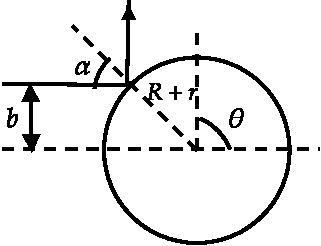
\includegraphics[height=3cm,width=4cm]{diagram-20220213-20220213123239-crop}
	\end{figure}
	\end{minipage}

			$$\text { where } \theta \text { is given by }(R+r) \sin \alpha=b \Rightarrow b=(R+r) \sin \left(\frac{\pi}{2}-\frac{\theta}{2}\right) \Rightarrow b=(R+r) \cos \frac{\theta}{2}$$
			The differential scattering cross section is
			\begin{align*}
			&D(\theta)=\frac{d \sigma}{d \Omega}=\frac{b}{\sin \theta}\left|\frac{d b}{d \theta}\right|=\frac{(R+r) \cos \frac{\theta}{2}}{\sin \theta} \cdot(R+r) \sin \frac{\theta}{2} \cdot \frac{1}{2}=\frac{(R+r)^{2}}{4} \\
			&\Rightarrow D(\theta)=\frac{d \sigma}{d \Omega}=\frac{(R+r)^{2}}{4}\\
			&\sigma=\int_{0}^{\pi} \int_{0}^{2 \pi} D(\theta) \sin \theta d \theta d \phi \Rightarrow \int_{0}^{\pi} \int_{0}^{2 \pi} \frac{(R+r)^{2}}{4} \sin \theta d \theta d \phi=\pi(R+r)^{2}
			\end{align*}	
	\end{answer}
	\begin{minipage}{\textwidth}
	\item If differential scattering cross-section is given by $D(\theta)=a^{2} \sin ^{2} \theta+b^{2} \cos ^{2} \theta$. If $N$ is the flux of incoming particle then find the number of scattered particle per unit time.
\end{minipage}
\begin{answer}
	\begin{align*}
	&\sigma=\int_{0}^{\pi} \int_{0}^{2 \pi} D(\theta) \sin \theta d \theta d \phi\\
		\sigma &=\int_{0}^{\pi} \int_{0}^{2 \pi} a^{2} \sin ^{2} \theta \sin \theta d \theta d \phi+\int_{0}^{\pi} \int_{0}^{2 \pi} b^{2} \cos ^{2} \theta \sin \theta d \theta d \phi \\
		&=2 \pi\left(a^{2} \int_{0}^{\pi} \sin ^{3} \theta d \theta+b^{2} \int_{0}^{\pi} \cos ^{2} \theta \sin \theta d \theta\right) \\
		\sigma &=2 \pi\left(\frac{4}{3} a^{2}+\frac{2}{3} b^{2}\right) \Rightarrow \sigma=\frac{4 \pi}{3}\left(2 a^{2}+b^{2}\right)
	\end{align*}
	$\text { Number of scattered particle } N_{S C}=N \sigma \Rightarrow N_{S C}=N \frac{4 \pi}{3}\left(2 a^{2}+b^{2}\right)$
\end{answer}
	\begin{minipage}{\textwidth}
	\item Yukawa potential is defined as $V(r)=\beta \frac{e^{-\mu r}}{r}$ where $\beta>0$ and $\mu>0$.\\
	(a) Using born approximation for for high energy $k=\sqrt{\frac{2 m E}{\hbar^{2}}}$ if $\theta$ is scattering angle with parameter $q=2 k \sin \theta / 2$ find differential scattering cross section\\
	(b) Discuss the differential scattering cross section for case $q \gg \mu$
\end{minipage}
\begin{answer}
	\begin{align*}
		\text { (a) } f(\theta)&=-\frac{2 m}{\hbar^{2} q} \int_{0}^{\infty} r V(r) \sin (q r) d r\\
		&=\frac{-2 m \beta}{\hbar^{2} q} \int_{0}^{\infty} e^{-\mu r} \sin (q r) d r\\&=\frac{-2 m \beta}{\hbar^{2} q} \frac{1}{2 i} \int_{0}^{\infty} e^{-\mu r} \exp i q r-\exp (-i q r) d r \\
		&\frac{-2 m \beta}{\hbar^{2} q} \frac{1}{2 i}\left(\int_{0}^{\infty} \exp -r(\mu-i q) d r-\int_{0}^{\infty} \exp -r(\mu+i q) d r\right)\\
		&=-\frac{m \beta}{i \hbar^{2} q}\left(\frac{1}{\mu-i q}-\frac{1}{\mu+i q}\right) \\
		&=-\frac{m \beta}{i \hbar^{2} q}\left(\frac{(\mu+i q)-(\mu-i q)}{\mu^{2}+q^{2}}\right)=-\frac{2 m \beta q}{\hbar^{2} q} \cdot \frac{1}{\mu^{2}+q^{2}}=-\frac{2 m \beta}{\hbar^{2}} \cdot \frac{1}{\mu^{2}+q^{2}} \\
		&D(\theta)=|f(\theta)|^{2}=\left|-\frac{2 m \beta}{\hbar^{2}} \cdot \frac{1}{\mu^{2}+q^{2}}\right|^{2}=\frac{4 m^{2} \beta^{2}}{\hbar^{4}} \cdot\left(\frac{1}{\mu^{2}+q^{2}}\right)^{2}
	\end{align*}
	(b) for case $q>>\mu$
	$$
	D(\theta)=\frac{4 m^{2} \beta^{2}}{\hbar^{4}} \cdot \frac{1}{q^{4}}\left(\frac{1}{(\mu / q)^{2}+1}\right)^{2}=\frac{4 m^{2} \beta^{2}}{\hbar^{4}} \cdot \frac{1}{q^{4}}
	$$
\end{answer}
	\begin{minipage}{\textwidth}
	\item A particle of energy $E$ scatters off a repulsive spherical potential
	$$
	V(r)=\left\{\begin{array}{ccc}
	V_{0} & \text { for } & r<a \\
	0 & \text { for } & r \leq a
	\end{array}\right.
	$$
	where $V_{0}$ and $a$ are positive constants. In the low energy limit, the total scattering crosssection is $\sigma=4 \pi a^{2}\left(\frac{1}{k a} \tanh k a-1\right)^{2}$, where $k^{2}=\frac{2 m}{h^{2}}\left(V_{0}-E\right)>0 .$\\
	(a) In the limit $V_{0} \rightarrow \infty$ find the total scattering cross section.\\
	(b) Compare the total scattering cross section from (a) to classical scattering cross section Consider the notentiol
\end{minipage}
\begin{answer}
	\begin{align*}
		\text { (a) } \sigma&=4 \pi a^{2}\left[\frac{1}{k a} \tanh k a-1\right]^{2}\\
	V_{0} \rightarrow \infty, k a \rightarrow \infty, \tanh k a \rightarrow 1 \Rightarrow \sigma&=4 \pi a^{2}\left(\frac{1}{k a}-1\right)^{2} \text { and } k a \rightarrow \infty, \lim _{k a \rightarrow \infty} \sigma=4 \pi a^{2}\\
	\text { (b) Classically } \sigma_{c}&=\pi a^{2}, \frac{\sigma}{\sigma_{c}}=4
	\end{align*}
\end{answer}
	\begin{minipage}{\textwidth}
	\item Consider the potential
	$$
	V(x, y, z)=\sum_{i} V_{0} a^{3} \delta\left(x-x_{i}\right) \delta\left(y-y_{i}\right) \delta\left(z-z_{i}\right)
	$$
	where $x_{i}, y_{i}, z_{i}$ are the position vectors of the vertices of a cube of length $a$ centered at the origin and $V_{0}$ is a constant. If $V_{0} a^{2}<<\frac{\hbar^{2}}{m}$ for low energy limit
	 \begin{tasks}(1)
		\task[\text{a)}] Find differential cross section .
		\task[\text{b)}]The total scattering cross-section
	\end{tasks}
\end{minipage}
\begin{answer}
	 $\sum_{i} V_{0} a^{3} \delta\left(x-x_{i}\right) \delta\left(y-y_{i}\right) \delta\left(z-z_{i}\right)$, where $x_{i}, y_{i}, z_{i}$ are co-ordinate at 8 corner cube whose center is at origin.\\
	 \begin{align*}
	 	f(\theta) &=-\frac{m}{2 \pi \hbar^{2}} \int V(r) d^{3} r \\
	 	&=\frac{-m}{2 \pi \hbar^{2}} V_{0} a^{3} \iint_{-\infty}^{\infty} \int \sum_{i=1}^{8} \delta\left(x-x_{i}\right) \delta\left(y-y_{i}\right) \delta\left(z-z_{i}\right) d x d y d z \\
	 	&=\frac{-m}{2 \pi \hbar^{2}} V_{0} a^{3}[1+1+1+1+1+1+1+1] \\
	 	&=\frac{-8 m V_{0} a^{3}}{2 \pi \hbar^{2}}=\frac{-4 m V_{0} a^{3}}{\pi \hbar^{2}}
	 \end{align*}
	 $\text { Differential scattering cross section } D(\theta)=|f(\theta)|^{2}=\frac{16 m^{2} V_{0}^{2} a^{6}}{\pi^{2} \hbar^{4}}$\\
	 (b) Total scattering cross section $\sigma=\int|f(\theta)|^{2} \sin \theta d \theta d \phi$.
	 \begin{align*}
	 &=\frac{16 m^{2} V_{0}^{2} a^{6}}{\pi^{2} \hbar^{4} \cdot 4 \pi}=\frac{64 a^{2}}{\pi}\left(\frac{m^{2} V_{0}^{2} a^{4}}{h^{4}}\right) \\
	 \sigma &=\frac{64 a^{2}}{\pi}\left(\frac{m V_{0} a^{2}}{\hbar^{2}}\right)^{2}
	 \end{align*}
\end{answer}

\end{enumerate}